\let\negmedspace\undefined
\let\negthickspace\undefined
\documentclass[journal,12pt,onecolumn]{IEEEtran}
\usepackage{cite}
\usepackage{amsmath,amssymb,amsfonts,amsthm}
\usepackage{algorithmic}
\usepackage{graphicx}
\usepackage{textcomp}
\usepackage{xcolor}
\usepackage{txfonts}
\usepackage{listings}
\usepackage{enumitem}
\usepackage{mathtools}
\usepackage{gensymb}
\usepackage{comment}
\usepackage[breaklinks=true]{hyperref}
\usepackage{tkz-euclide} 
\usepackage{listings}
\usepackage{gvv}                                        
\def\inputGnumericTable{}                                 
\usepackage[latin1]{inputenc}                                
\usepackage{color}                                            
\usepackage{array}                                            
\usepackage{longtable}                                       
\usepackage{calc}                                             
\usepackage{multirow}                                         
\usepackage{hhline}                                           
\usepackage{ifthen}                                           
\usepackage{lscape}

\newtheorem{theorem}{Theorem}[section]
\newtheorem{problem}{Problem}
\newtheorem{proposition}{Proposition}[section]
\newtheorem{lemma}{Lemma}[section]
\newtheorem{corollary}[theorem]{Corollary}
\newtheorem{example}{Example}[section]
\newtheorem{definition}[problem]{Definition}
\newcommand{\BEQA}{\begin{eqnarray}}
\newcommand{\EEQA}{\end{eqnarray}}
\newcommand{\define}{\stackrel{\triangle}{=}}
\theoremstyle{remark}
\newtheorem{rem}{Remark}
\begin{document}

\bibliographystyle{IEEEtran}
\vspace{3cm}

\title{11.15}
\author{EE23BTECH11029 - Kanishk}
\maketitle

\bigskip

\renewcommand{\thefigure}{\theenumi}
\renewcommand{\thetable}{\theenumi}
\footnotesize
\textbf{Question}:\\ 

A SONAR system fixed in a submarine operates at a frequency 40.0 kHz. An enemy submarine moves towards the SONAR with a speed of 360 km/hr. What is the frequency of sound reflected by the submarine? Take the speed of sound in water to be 1450 m/s.\\

\textbf{Solution}:\\


\begin{tabular}{|c|c|c|}
   
   \hline
   Parameter & Description & Value\\
   \hline
   $V $& Speed of sound in water & 1450m/s\\
   \hline 
   $V_e$ & Speed of enemy submarine & 100m/s\\
   \hline 
   $Vrel$ & Relative velocity between both submarine & 1550m/s\\
   \hline
   $f $& Frequency of SONAR wave & 40kHz\\ 
   \hline
   $y\brak{x,t}$ & Equation of SONAR wave & $A\sin\brak{2\pi ft-\frac{2\pi}{\lambda}x+\phi}$\\
   \hline
   $\lambda$ & Wavelength of SONAR wave & 3.625cm\\
    \hline
   $ f' $& Frequency observed by enemy submarine & 42.76kHz\\
   \hline
   $\lambda_2$ & Wavelength of reflected wave & 3.157cm\\
   \hline 
   $T=\frac{1}{f'}$ & Time period of reflected wave & 23.38s\\
   \hline
  $ y_2\brak{x,t}$ & Equation of reflected wave as observed from submarine& $A\sin\brak{2\pi f''t-\frac{2\pi}{\lambda_2}x+\phi}$\\
   \hline
   
\end{tabular}   
\\
\\
\\
Let us assume that the wave is reflected completely from enemy submarine.\\
The source(SONAR system) is at rest and the observer (enemy submarine) is moving toward it. \\
Enemy submarine(observer) is approaching the SONAR(source), So 

\begin{equation}
Vrel=V+V_e
\end{equation}
Frequency observed by the enemy submarine would be
\begin{align}
f'&=Vrel/\lambda\\
&=\brak{\frac{V+Ve}{V}}f\\
&= \brak{\frac{1450+100}{1450}}40\\
&=42.76kHz
\end{align}

This frequency (f') is reflected by the enemy ship and is observed by the SONAR (which now acts as observer).
Now the the enemy submarine has become source,\\
In time period T the wave reflected by source(enemy submarine) will travel distance VT and source will travel by distance $V_eT$\\
So the change in displacement by the wave and source would be the wavelength of the wave
\begin{align}
\lambda_2&=T\brak{V-V_e}\\
&=\brak{\frac{V-V_e}{f'}}\\
f''&=V/\lambda_2\\
&=\brak{\frac{V}{V-V_e}}f'
\end{align}
\\
\begin{tabular}{|c|c|c|}
   \hline
   Parameter & Description & Value\\
   \hline
   $f''= \brak{\frac{V}{V-V_e}}f'$& Frequency of reflected wave & 45.93kHz\\
   \hline
   
\end{tabular}
\newpage
Let us assume that amplitude of both waves is 1 , So graph of waves are given as: 

\begin{figure}[h]
   
    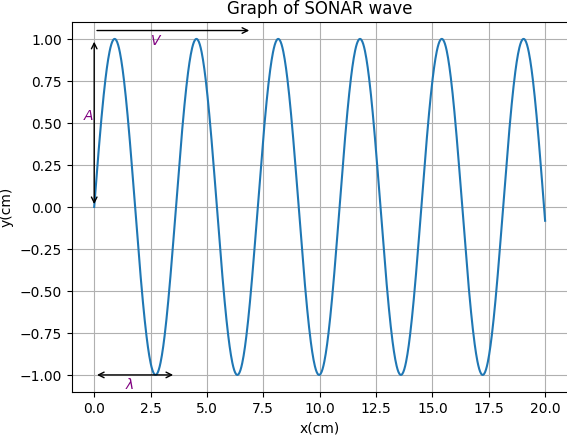
\includegraphics[width=120mm]{figs/fig1.png}\\
     \centering
    {Fig. 1}
  
\end{figure}

\begin{figure}[h]
    
    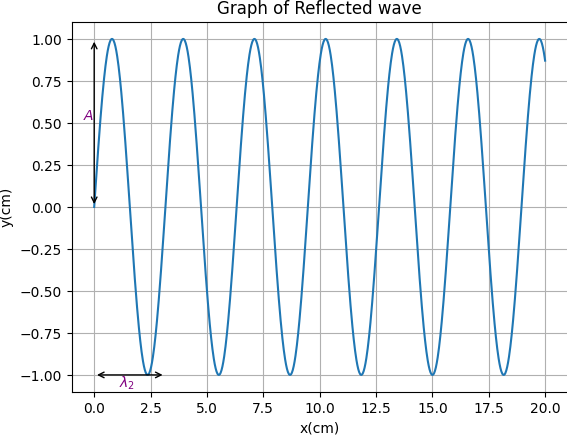
\includegraphics[width=120mm]{figs/fig2.png}\\
     \centering
    {Fig. 2}
\end{figure}

\end{document}



  



